\documentclass{article}
\usepackage{tikz}
\usepackage{CJKutf8}
\usepackage{amsmath}
\usepackage{amsthm}
\renewcommand{\figurename}{图}
\begin{document}
\begin{CJK}{UTF8}{gbsn}
  \newtheorem{Th1}{定理}
  \newtheorem{Th2}{定理}
  \begin{Th1}
  设树$T$有$p$个顶点,$q$条边,则$q = p-1$。(数学归纳法I,数学归纳法II)
  \end{Th1}
  \begin{Th1}
  如果有$p$个顶点$q$条边的平面连通图$G$有$f$个面,则$p - q + f = 2$。(数学归纳法I)
\end{Th1}
\begin{Th1}
  若$G$为一个有$p$个顶点$q$条边的可平面图,$p\geq 3$,则$q \leq 3p - 6$。
  (直接证明法)
\end{Th1}
\begin{Th1}
      $K_5$不是可平面图。(反证法)
\end{Th1}
\begin{Th1}
每个可平面图$G$中顶点度的最小值不超过5,即$\delta (G) \leq 5$。(直接证明法,反证法)   
\end{Th1}
\begin{Th1}
  每个可平面图是$5-$可着色的。    (数学归纳法II)
\end{Th1}
\begin{Th2}
  设树$T$有$p$个顶点,$q$条边,则$q = p-1$。
\end{Th2}
\begin{proof}[证明(证法一)]
  \mbox{}\par{}
    用数学归纳法证明,施归纳于顶点数$p$。
    
    (1)当$p=1$时,$q=0$,结论显然成立。

    (2)假设当$p=k$时结论成立,往证当$p=k+1$时结论也成立。设树$T$有$k+1$个顶点。$T$中一定存在一个度为1的顶点,这是因为,设$P$为$T$中的一条最长路,$v$为$P$的一个端点,则$v$除了$P$上与其关联的边之外,由$T$中无圈知$v$不能再有其他的与$P$上的顶点相关联的边,同时由$P$为一条最长路知$v$不能再有与$P$外的顶点相关联的边,因此$v$的度必为1。去掉$T$中一个度为1的顶点及其与之关联的边,得到的图$T'$连通且无圈,则$T'$是树。$T'$有$k$个顶点,$q-1$条边,由归纳假设,$q-1 = k - 1$,从而$q = (k +1) - 1$,即当$p=k+1$时结论也成立。
\end{proof}
\begin{proof}[证明(证法二)]
\mbox{}\par{}
      用数学归纳法证明,施归纳于边数$q$。
    
    (1)当$q=0$时,$p=1$,结论显然成立。

    (2)假设当$q<k$时结论成立,往证当$q=k$时结论也成立。设树$T$有$k$条边。去掉$T$中的任意一条边,得到两个支$T_1$和$T_2$,它们均连通无圈,因此是树。设$T_1$有$p_1$个顶点,$k_1$条边,$T_2$有$p_2$个顶点,$k_2$条边,由归纳假设,
    \begin{equation*}
      \begin{split}
        k_1 &= p_1 - 1\\
        k_2 &= p_2 - 1
      \end{split}
    \end{equation*}
    以上两式相加,两边再同时加1,得
    \[k_1 + k_2  + 1 = p_1 + p_2 - 1\]
    从而
    \[k = p - 1 \]
    即当$q=k$时结论也成立。
\end{proof}

\begin{Th2}
如果有$p$个顶点$q$条边的平面连通图$G$有$f$个面,则$p - q + f = 2$。
\end{Th2}
\begin{proof}[证明]
    用数学归纳法证明,施归纳于面数$f$。

  (1)当$f=1$时,$G$中无圈,又因为$G$是连通的,所以$G$是树。从而
  $q=p-1$,$p-q+f=2$成立。

  (2)假设当$f=k(k\geq 1)$时结论成立,往证当$f=k+1$时结论也成立。假设$G$有$k+1$个面,此时$G$至少有一个内部面,从而有一个圈。从这个圈上去掉一条边$x$,则
  $G-x$就是一个有$p$个顶点,$q-1$条边,$k$个面的平面连通图。由归纳假设,对
  $G-x$结论成立,即\[p-(q-1) + k =2\]
  因此,\[p-q+ (k+1) =2\]
  即当$f=k+1$时结论也成立。
\end{proof}

\begin{Th2}
若$G$为一个有$p$个顶点$q$条边的可平面图,$p\geq 3$,则$q \leq 3p - 6$。
\end{Th2}
\begin{proof}[证明]
  不妨设$G$为连通的可平面图,否则可以加边使之变成连通的。由于每个面至少含有3条边,因此
  \[2q \geq 3f\]
  即
  \[\frac{2q}{3} \geq f\]
  因此,根据欧拉公式
  \[p - q + f = 2\]
  得
  \[p - q + \frac{2q}{3} \geq 2\]
  化简得:
  \[q \leq 3p - 6\]
\end{proof}

\begin{Th2}
      $K_5$不是可平面图。
\end{Th2}
\begin{proof}[证明]
  用反证法。假设$K_5$是可平面图,其顶点数$p = 5$, 边数$q = 10$,此时
  \[q \leq 3p - 6\]
  即
  \[10 \leq 3 \times 5 - 6 = 9\]
  矛盾。因此$K_5$不是可平面图。
\end{proof}
    
\begin{Th2}
每个可平面图$G$中顶点度的最小值不超过5,即$\delta  \leq 5$。   
\end{Th2}
\begin{proof}[证明(证法一)]
  当图$G$的顶点数$p=1,2$时,结论显然成立。当$p\geq 3$时,
  设可平面图$G$有$q$个顶点,则
  \[\delta p \leq 2q\]
  由$G$为可平面图知
  \[q \leq 3p - 6\]
  从而
  \[\delta p \leq 6p - 12\]
  两边同时除以$p$,得:
  \[\delta \leq 6 - \frac{12}{p}\]
  即
  \[\delta \leq 5\]
\end{proof}
\begin{proof}[证明(证法二)]
  当图$G$的顶点数$p=1,2$时,结论显然成立。
  当$p \geq 3$时,用反证法证明结论也成立。假设$\delta \geq 6$,则
  \[6p \leq 2q\]
  由$G$为可平面图知
  \[q \leq 3p - 6\]
  从而
  \[6p \leq 6p - 12\]
矛盾。  
\end{proof}
\begin{Th2}
  每个可平面图是$5-$可着色的。
\end{Th2}
\begin{proof}[证明]
  用数学归纳法证明,施归纳于图的顶点数$p$。

  (1)当$p=1$时,结论显然成立。

  (2)假设当$p<k$时结论成立,往证当$p=k$时结论也成立。设平面图$G$有$k$个顶点,则图$G$中一定有一个顶点$v$使得$\deg v \leq 5$。于是,$G-v$是一个有$k-1$个顶点的平面图,由归纳假设,$G-v$是$5-$可着色的。假设用至多5种颜色对$G-v$进行了着色。

  如果$\deg v \leq 4$,则在$G-v$中用至多5种颜色进行顶点着色时,在$G$中与$v$邻接的顶点至多用了$4$种颜色,如图\ref{fig:coloring}所示,用另外一种不同的颜色对顶点$v$进行着色,这样用至多5种颜色就可以对$G$的顶点进行着色,从而图$G$是$5-$可着色的。

\begin{figure}
  \begin{minipage}{0.49\linewidth}
    \centering
   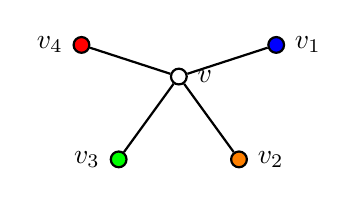
\begin{tikzpicture}[auto,
    specification/.style ={circle, draw, thick, inner sep = 0pt, minimum size=2mm}]
   \node[specification, fill = blue] (A)  [label=0:$v_1$] at (18:1.3cm)  {};
   \node[specification, fill = red] (C)  [label=180:$v_4$] at (162:1.3cm)  {};
   \node[specification, fill = green] (D) [label=180:$v_3$] at (234:1.3cm)  {};
   \node[specification, fill = orange] (E)  [label=0:$v_2$] at (306:1.3cm)  {};      
   \node[specification] (o)  [label=0:$v$] at (0,0)  {};      
   \draw[thick] (A) to  (o);
   \draw[thick] (C) to  (o);
   \draw[thick] (D) to  (o);
   \draw[thick] (E) to  (o);
 \end{tikzpicture}
    \caption{$\deg v \leq 4$的情况}
    \label{fig:coloring}  
  \end{minipage}
  \begin{minipage}{0.49\linewidth}
    \centering
   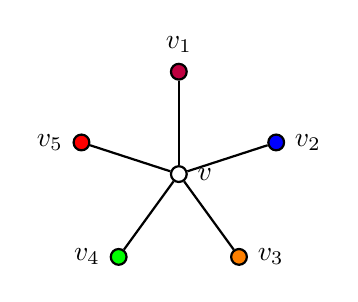
\begin{tikzpicture}[auto,
    specification/.style ={circle, draw, thick, inner sep = 0pt, minimum size=2mm}]
   \node[specification, fill = blue] (A)  [label=0:$v_2$] at (18:1.3cm)  {};
   \node[specification, fill = purple] (B)  [label=90:$v_1$] at (90:1.3cm)  {};
   \node[specification, fill = red] (C)  [label=180:$v_5$] at (162:1.3cm)  {};
   \node[specification, fill = green] (D) [label=180:$v_4$] at (234:1.3cm)  {};
   \node[specification, fill = orange] (E)  [label=0:$v_3$] at (306:1.3cm)  {};      
   \node[specification] (o)  [label=0:$v$] at (0,0)  {};      
   
   
   \draw[thick] (A) to  (o);
   \draw[thick] (B) to  (o);
   \draw[thick] (C) to  (o);
   \draw[thick] (D) to  (o);
   \draw[thick] (E) to  (o);
 \end{tikzpicture}
  \caption{$\deg v = 5$的情况}
  \label{fig:collision}
  \end{minipage}
\end{figure}    


  如果$\deg v = 5$,与$v$邻接的$5$个顶点$v_1,v_2,v_3,v_4,v_5$在$G-v$中用$c_1,c_2,c_3,c_4,c_5$ 5种颜色进行了着色。如果$c_1,c_2,c_3,c_4,c_5$中有两种颜色是相同的,则$c_1$, $c_2$, $c_3$, $c_4$, $c_5$中至多有$4$种颜色,用另一种颜色对顶点$v$进行着色,这样用至多5种颜色就可以对$G$的顶点进行着色。以下考虑$c_1,c_2,c_3,c_4,c_5$中的各种颜色互不相同的情况,如图\ref{fig:collision}所示。在图$G$中,与顶点$v$邻接的$5$个顶点$v_1,v_2,v_3,v_4,v_5$中一定有两个顶点是不邻接的,否则图$G$中将有一个子图$K_5$,这与图$G$为平面图相矛盾。取其中不邻接的两个顶点$v_i$和$v_j$,在$G-v$中,将顶点$v_i$和顶点$v_j$视为同一个顶点$w$,即去掉顶点$v_i$和$v_j$,添加一个新的顶点$w$,原来与顶点$v_i$和顶点$v_j$相关联的边变为与顶点$w$相关联的边,得到的新的图记为$G'$,则$G'$仍然是平面图。由归纳假设,$G'$是$5-$可着色的。 设用至多$5$种颜色对$G'$进行了顶点着色。在$G-v$中,顶点$v_i$和顶点$v_j$都着与$w$相同的颜色,其他的顶点均与$G'$中相对应的顶点着相同的颜色,这样$G-v$用至多5种颜色就可以进行顶点着色。在这里,在$G$中与顶点$v$邻接的五个顶点$v_1,v_2,v_3,v_4,v_5$中用了4种颜色,用另外一种颜色对顶点$v$着色,这样用至多5种颜色就可以对$G$的顶点进行着色,从而图$G$是$5-$可着色的。

  
\end{proof}
\end{CJK}
\end{document}

%%% Local Variables:
%%% mode: latex
%%% TeX-master: t
%%% End:
